\chapter{Electrically Detected Electron Paramagnetic Resonance on a Cathode of an Organic Radical Battery}

\paragraph*{}
With EDMR we observe the hopping charge as it travels to the charge bearing group through the electrode.

\section{Distribution of Current Density in On-Substrate Meander-Shaped Electrodes}
Meander-shaped electrodes shown in Figure~\ref{fig:grid} are used to study properties of thin conductive films. The distribution of electric potential and the current within a film of poor conductivity and a finite thickness be not obvious. 

\begin{figure} [!ht]
\begin{center}
       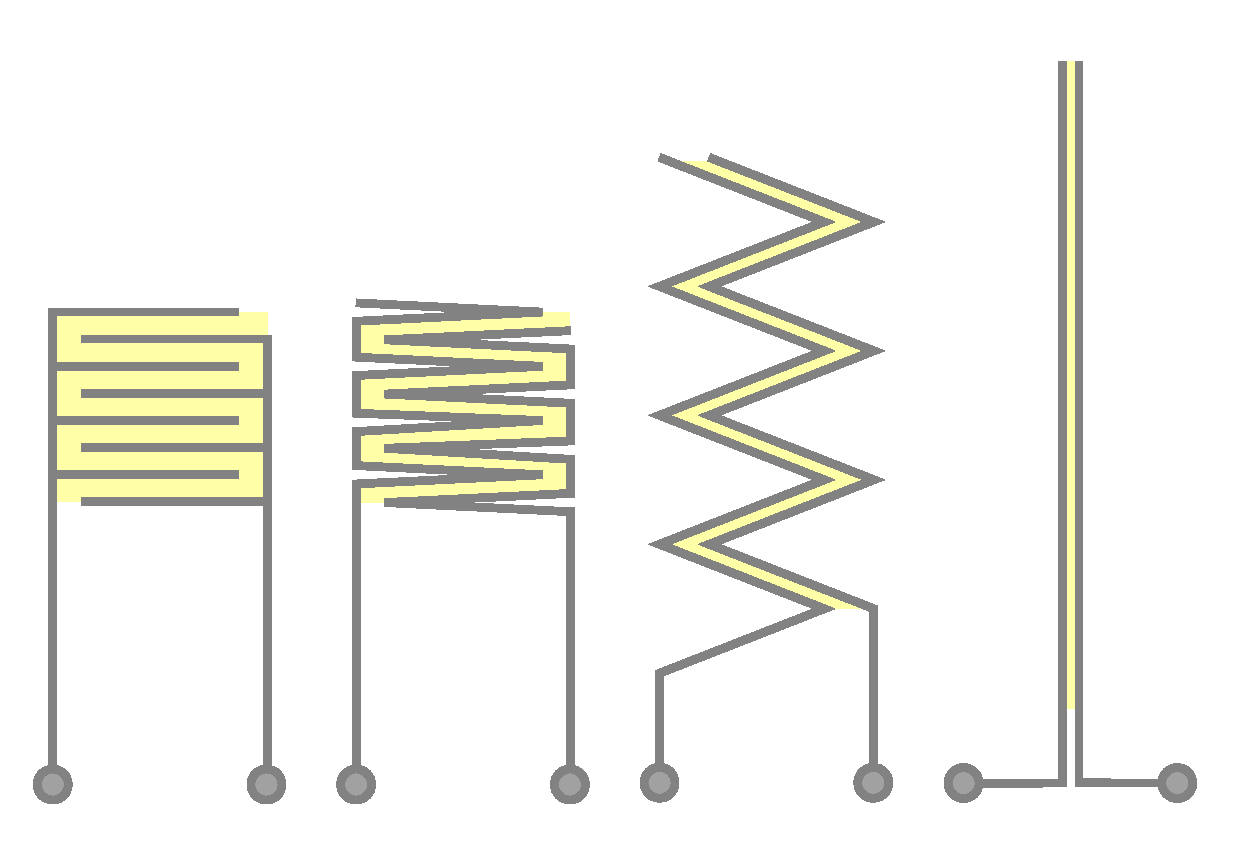
\includegraphics[width=0.5\textwidth]{./edmr/fingers1/pics/grid.pdf}
       \end{center}
\caption{Transformation of the meander-shaped electrode grid into two linear electrodes}
     \label{fig:grid}
\end{figure}

A numerical solution was found to the distribution of the current density $\vec{j}$ within a film of a finite thickness, connected by two metal electrodes. Two cases were considered, a thick film and a thin film.

\begin{figure} [!ht]
\begin{center}
       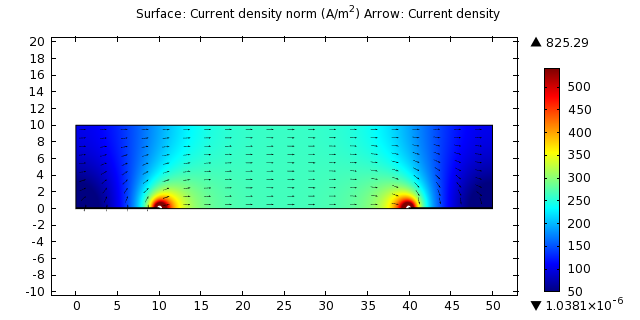
\includegraphics[width=0.5\textwidth]{./edmr/fingers1/pics/3_thick_film.png}
       \end{center}
\caption{Distribution of electric current in a thick polymer film. The current is uniform in the middle of the film. \raw{Let us see, whether we can apply the simple, bulk formula to this structure.}}
     \label{fig:dits_thick_2d}
\end{figure}

\begin{figure} [!ht]
\begin{center}
       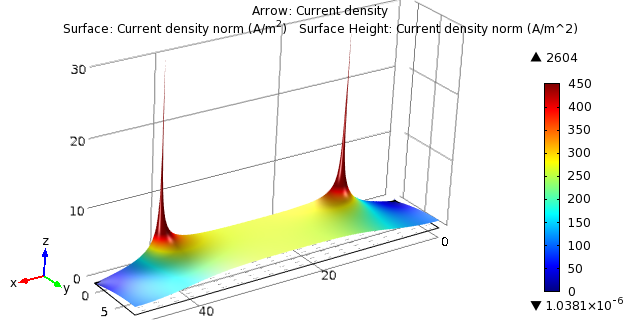
\includegraphics[width=0.5\textwidth]{./edmr/fingers1/pics/3_thick_film_2.png}
       \end{center}
\caption{Thick film. The current is uniform in the middle of the film. It is better seen on this 3d plot. Let us see, whether we can apply the simple, bulk formula to this structure. \raw{I think we do not gain a lot of error by saying that the current is uniform within the whole film.}}
     \label{fig:dits_thick_3d}
\end{figure}


\begin{figure} [!ht]
\begin{center}
       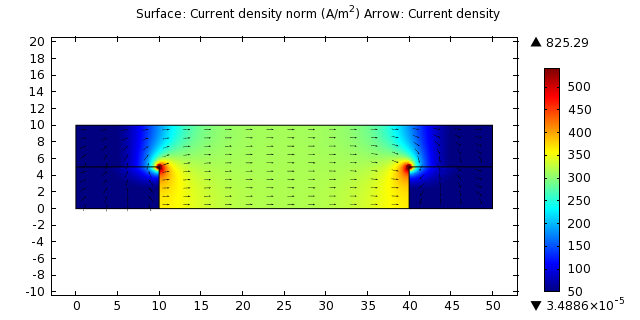
\includegraphics[width=0.5\textwidth]{./edmr/fingers1/pics/2_intermediate_film.png}
       \end{center}
\caption{Distribution of electric current in an intermediate polymer film}
     \label{fig:dits_inter}
\end{figure}

\begin{figure} [!ht]
\begin{center}
       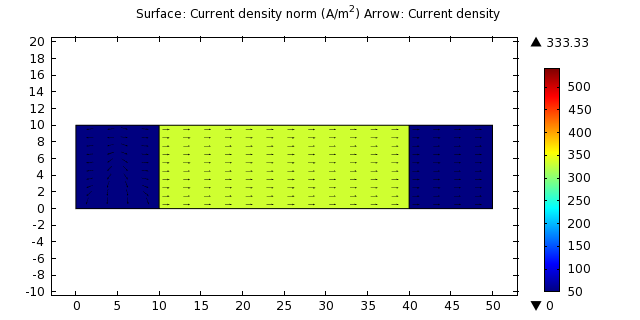
\includegraphics[width=0.5\textwidth]{./edmr/fingers1/pics/1_thin_film.png}
       \end{center}
\caption{Distribution of electric current in a thin polymer film}
     \label{fig:dits_thin}
\end{figure}

\begin{figure} [!ht]
\begin{center}
       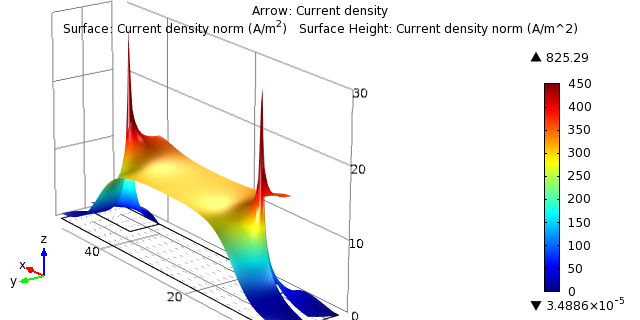
\includegraphics[width=0.5\textwidth]{./edmr/fingers1/pics/3_intermediate_film_2.png}
       \end{center}
\caption{Very high values of the computed distribution of the current density in a film of intermediate thickness due to the sharp edges of the contacts.}
     \label{fig:dits_singular}
\end{figure}


